\section{Spezifische Anforderungen}
\subsection{Funktionale Anforderungen}
\subsubsection{DFD1 Simulation}
\begin{figure}[H]
	\centering
  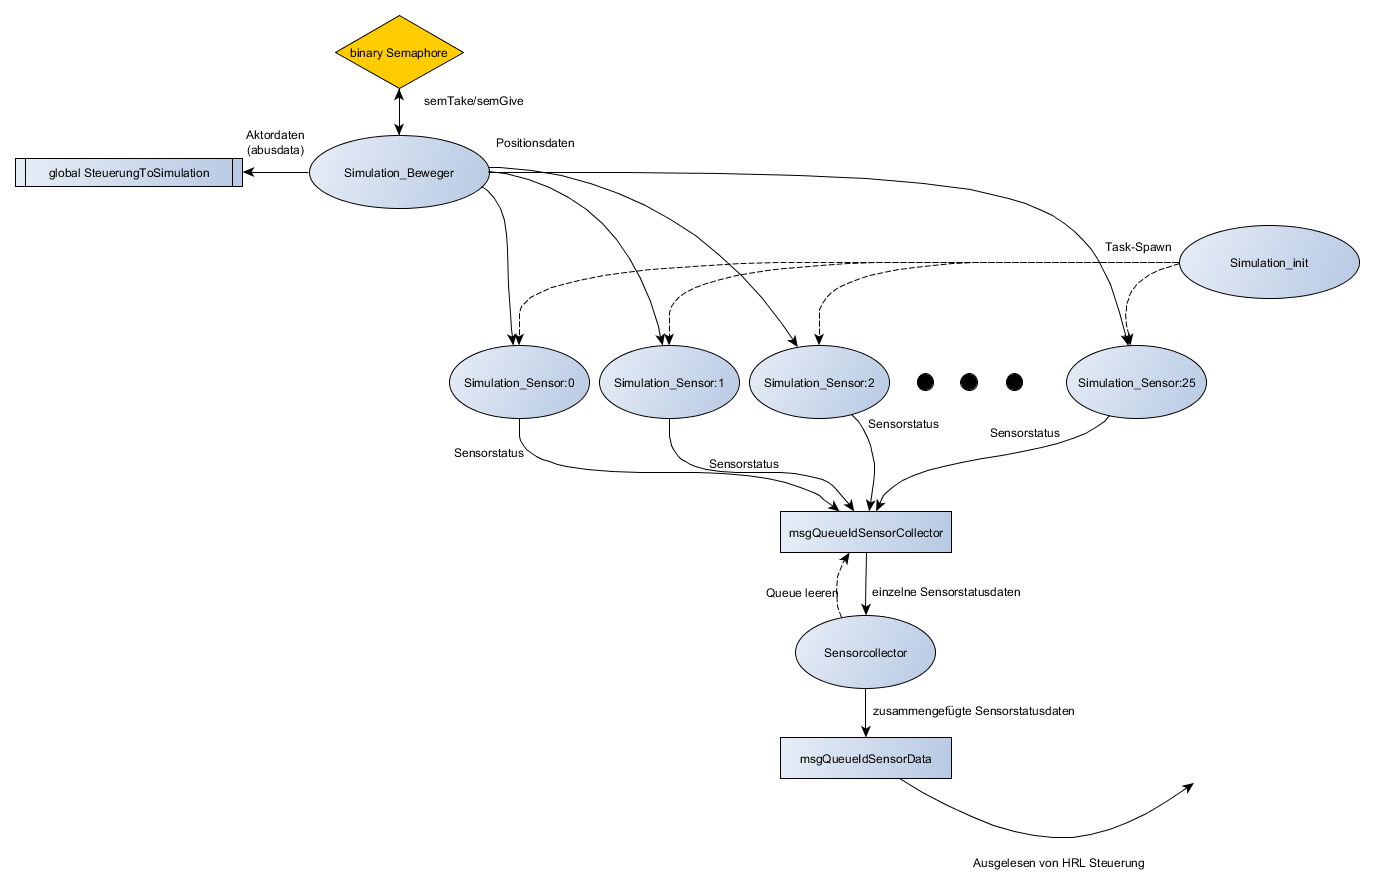
\includegraphics[width=\textwidth]{DFD/dfd1_simulation1_1.png}
	\caption{DFD1 Simulation}
	\label{fig1}
\end{figure}
\begin{figure}[H]
	\centering
  \includegraphics[width=\textwidth]{diagrams/gand.png}
	\caption{Gantt Diagramm der Task der Simulation}
	\label{gantt}
\end{figure}

\paragraph{Beweger}
Wie in Abb.\ref{gantt} zu sehen ist läuft der \textbf{Beweger} als erster Task eines Simulationsschrittes. Zuerst aktualisiert er die Aktorwerte aus der gloablen Variable \textbf{AktorBusData}. Diese entspricht den Busdaten \todo{entspricht was?} und ist durch einen Semaphor geschützt. Da die Simulation minimal blockiert werden soll implementiert der Semaphor Prioritätsvererbung. Daraufhin \glqq verschiebt\grqq er den Turm entsprechend den Aktordaten.

\paragraph{Sensorcollector}
Der \textbf{Sensorcollector} sammelt aus der \textbf{MessageQueue} die Einträge aller Sensoren. Wenn ein Sensor ausfällt bleibt der Wert des Sensors auf 1.

\paragraph{Simulation Sensor x}
Jeder Sensor bekommt eine id übergeben die seine Funktion und ihn eindeutig definiert. 
\begin{enumerate}
\item \textbf{Tastsensoren} überprüfen ob die Turmposition mit der Sensorposition übereinstimmt.
\item \textbf{Lichtschranken} Simulieren entweder das eintreffen eines Klötzchens am Eingabeslot oder das Entfernen eines Klötzchens am Ausgabeslot, jeweils mit einem vordefinierten Delay. \todo{Das könnte besser sein}
\item Der \textbf{Lichttaster} im Turm wird dann ausgelöst wenn die vorige y-Position des Turms im vorigen Schritt über (beim Ablegen eines Klötzchens) bzw. unter (beim Aufnehmen) der jetzigen Position ist und (beim Ablegen) ein Klötzchen im Turm ist bzw. (beim Aufnehmen) ein Klötzchen an der Aufnahmeposition ist.

\end{enumerate}
\begin{table}[h]
\centering
\begin{tabular}{|l|r|}
\hline
Taster X[0-9] &  [gedrückt|gehalten] \\
\hline
Taster Y[0-9] &  [gedrückt|gehalten] \\
\hline
Taster Z[0-3] &  [gedrückt|gehalten] \\
\hline
Lichtschranke Eingabe & [unterbrochen|nicht unterbrochen] \\
\hline
Lichtschranke Ausgabe & [unterbrochen|nicht unterbrochen] \\
\hline
Turmlichtschalter & [bedeckt|nicht bedeckt]\\
\hline
\end{tabular}
\caption{Requirements Dictionary}
\label{tab:Requirements Dictionary}
\end{table}
